\chapter{Tests}
Diese Testdokumentation wurde erstellt, um die Herangehensweise, Durchführung sowie die Ergebnisse unseres Testprozesses festzuhalten. 

\section{Ziele}
Ziel unseres Testprozesses ist es garantieren zu können, dass die in diesem Projekt geschaffene Software unter den von uns festgelegten Vorraussetzungen annähernd bis vollständig fehlerfrei und mit möglichst guter Performance betrieben werden kann. Auffälligkeiten sowie nach dem Testprozess bekannte und nicht behobene Fehler sollen am Ende des Testprozesses dokumentiert sein.

\section{Rahmenbedingungen}
Grundsätzlich wurde während der Entwicklung der Anwendung stets darauf geachtet, dass die jeweils neu implementierten Features einwandfrei funktionieren und auch, dass durch die Implementierung jener Features keine der zuvor vorhandenen Teile beschädigt werden. Dennoch haben wir in unserer Projektplanung eine gesonderte Testphase geplant, bei der wir im Zeitraum von zwei Wochen alle nötigen Schritte abschließen möchten, um die von uns erstellte Anwendung ausgiebig zu testen. In dieser zweiwöchigen Testphase soll der Testprozess vollständig abgeschlossen werden. Alle einzelnen Tests von Fron-End sowie Back-End wurden dabei jeweils in der selben Testumgebung durchgeführt.

\section{Teststrategie}
Um unser Testziel zu erreichen greifen wir auf verschiedene Testmethoden zurück. Da die Testphase sowohl durch einen kurzen Zeitraum, als auch die Anzahl der Tester eingeschränkt ist, müssen wir diese Ressourcen bestmöglich nutzen. Nach längeren Diskussionen innerhalb des Entwicklungsteams haben wir uns dazu entschlossen, auf eine Kombination von automatisierten Unit-Tests, manuellen System- und UI-Tests, sowie Last-Test zu setzen. Auf diese Weise decken wir beim Testen nicht nur funktionale sondern auch qualitative Anforderungen der Software ab.

Welche Methodik bei den einzelnen Teilen der Anwendung verwendet wurde wird in der folgenden Tabelle \ref{testarten_software} dargestellt.

\begin{table}[]
	\begin{tabular}{|l|l|}
		\cline{1-2}
		\textbf{Testobjekt} & \textbf{Art des Testens} \\ \cline{1-2}
		Front-End           & \begin{tabular}[c]{@{}l@{}}Unit-Tests,\\ Manuelle Tests\end{tabular} \\ \cline{1-2}
		Back-End            & \begin{tabular}[c]{@{}l@{}}Unit-Tests.\\ Manuelle Tests\end{tabular} \\ \cline{1-2}
		Gesamtsystem        & \begin{tabular}[c]{@{}l@{}}Manuelle Tests,\\ Last-Tests\end{tabular} \\ \cline{1-2}
	\end{tabular}
\caption{Testarten der unterschiedlichen Softwareteile}
\label{testarten_software}
\end{table}

Trotz dessen, dass wir eine eigene Testphase geplant haben, ist es uns wichtig über den gesamten Entwicklungsprozess der Software für eine stets einwandfrei lauffähige Anwendung zu sorgen. Dies entspricht nicht nur unserem agilen Softwareentwicklungsprozess nach Scrum, sondern erleichtert auch die gemeinsame Arbeit durch mehrere Entwickler jeweils an Front-End sowie Back-End. Um dies gewährleisten zu können, haben wir abseits der Testphase jedes neu implementierte Feature sowie die Auswirkungen der Implementierung auf den Rest der Anwendung manuell getestet.

\section{Testen des Front-Ends}

\subsection{Unit-Tests}
Bei unserem Front-End sind wir zu dem Schluss gekommen, dass ein automatisiertes Testen nur bedingt sinnvoll ist. Ein großer Teil der Implementierungen dort bezieht sich rein auf die Darstellung der vom Back-End erhaltenen Daten im Webbrowser, oder um das Beschaffen und Versenden eben dieser Daten. Ein automatiertes Testen der Weboberfläche ist dabei überproportional aufwändig und in unserem Falle in den meisten Fällen nicht sinnvoll, da es sich vor allem um statische Inhalte oder um Video- beziehungsweise Bildinhalte handelt. Außerdem muss beim Testen einer Weboberfläche auf Faktoren wie Browserkompatibilität geachtet werden, was durch manuelles Testen besser umsetzbar ist. Nichts desto trotz wurde für jede Komponente des Front-Ends ein eigener Unit-Test erstellt, der die vollständige Erzeugung eben dieser Komponente simuliert und testet. Dabei werden für die Komponente erforderliche Abhängigkeiten durch Mock-Objekte ersetzt, um ein unabhängiges Testen zu ermöglichen.

Standardgemäß verwenden wir beim automatisierten Testen unseres Angular-Front-Ends das Testframework Karma. Dieses ist bereits beim Erzeugen eines neuen Angular-Projektes per Angular-\acs{CLI} integriert und vorkonfiguriert. 

\subsubsection{Ausführen der Unit-Tests}
Nachdem das Projekt korrekt auf die in \ref{chapter_installation} Dargestellte Art und Weise installiert wurde und lauffähig ist, können die automatisierten Tests durch das Aufrufen eines Konsolenbefehls gestartet werden. Dazu muss im Projektordner ein Terminal geöffnet werden und der Befehl \glqq{}ng test\grqq ausgeführt werden.

\subsubsection{Ergebnisse der Unit-Tests}

\begin{figure}[ht]
	\flushright
	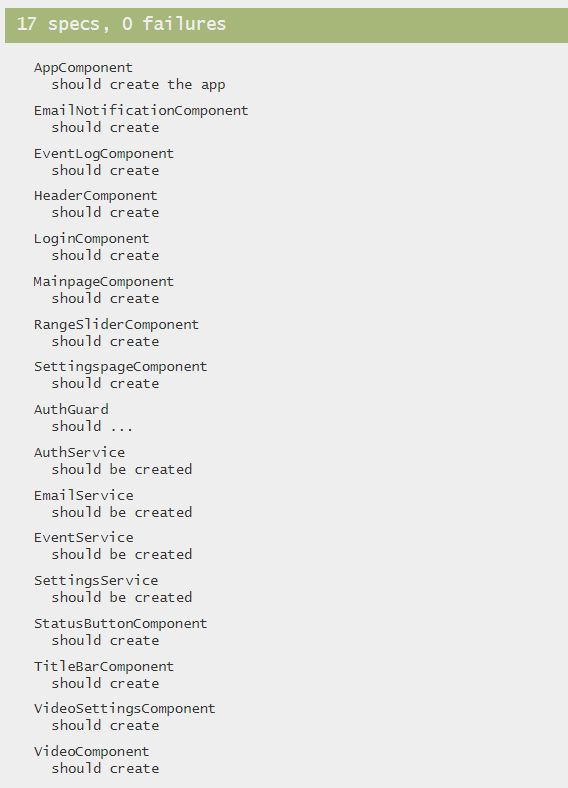
\includegraphics[]{content/pictures/ErgebnisseAutomatisierteTestsFrontend.jpg}
	\caption{Ergebnisse der automatisierten Front-End-Tests}
	\label{fig:ergebnisse_autom_tests_frontend}
\end{figure}


\subsection{Manuelle Tests}
\label{subsection_manuelle_tests}
Beim manuellen testen handelt es sich um einen Testprozess, bei dem der Tester ohne die Verwendung von Automatisierungstools vorgeht. Dabei können durch die systematische Verwendung der Software und das Nutzen von Diagnosetools oft Fehler aufgedeckt werden, die etwa bei Unit-Tests häufig nicht gefunden werden. Insbesondere Benutzeroberflächen können auf diese Weise unkompliziert getestet werden.

Im folgenden wird tabellarisch festgehalten, welche Aktionen getestet wurden und von welcher Ausgangssituation aus getestet wurde. Alle Tests wurden in den beiden Browsern Google Chrome (64-Bit Version 71.0.3578.98 Offizieller Build) und Mozilla Firefox (64-Bit Version 63.0.1 Offizieller Build) auf einem mit Windows 10 betriebenem Laptop mit einer Auflösung von 1920x1080 durchgeführt.

\vspace{0.5cm}

Vorraussetzung für alle Tests ist selbsterklärend, dass Front-End sowie Back-End korrekt installiert und gestartet sind. Zudem sind alle Einstellungen sinnvoll gewählt. Das bedeutet beispielsweise, dass ein funktionierender MJPEG-Stream hinterlegt ist. Es sind außerdem fünf beliebige Clips mit allen nötigen Werten korrekt gespeichert sowie abrufbar. Es sind auch zwei E-Mail-Adressen gespeichert.

\vspace{0.5cm}

Folgende Einstellungen waren bei den folgenden manuellen Tests vorhanden:

\begin{longtable}{| p{.2\textwidth} | p{.6\textwidth} |}
	\hline
	\textbf{Einstellung} & \textbf{Wert} \\ \hline

	sensitivity & 0.0 \\ \hline
		
	brightness & 0.5 \\ \hline
		
	contrast & 1.0 \\ \hline
		
	global\_notify & true \\ \hline
		
	log\_enabled & true \\ \hline
		
	streamaddress & https://webcam1.lpl.org/axis-cgi/mjpg/video.cgi \\ \hline
		
	cliplength & 10 \\ \hline
		
	max\_logs & 20 \\ \hline
		
	max\_storagee & 1024 \\ \hline
	
\caption{Eingestellte Werte vor jedem manuellen Test}
\label{tab:eingestellte_werte_vor_tests}
\end{longtable}

Alle manuellen Tests des Front-Ends inklusive deren Ergebnisse können im Anhand A eingesehen werden.

\section{Testen des Back-Ends}
Für das Testen der für das Back-End erstellten Tests wurde eine Testsuite angelegt, welche alle Testklassen auf einmal ausführt.
\subsection{Webserver}
Für alle Schnittstellen wurden Tests angelegt und mindestens auf Verfügbarkeit geprüft (Tabelle \ref{table:test-webserver}).

\begin{table}[h]
	\centering
	\caption{Unittests für Webserver}
	\label{table:test-webserver}
	\resizebox{\textwidth}{!}{\begin{tabular}{llll}
\textbf{Testname}                      & \textbf{Testmethode}    & \textbf{Eingabe}                                                                                                                   & \textbf{Ausgabe}               \\
test\_login\_wrong                     & post /login             & \{'user': 'user', 'password': 'bla'\}                                                                                              & Statuscode == 403              \\
test\_login\_wrong\_empty              & post /login             & \{\}                                                                                                                               & Statuscode == 403              \\
test\_login\_correct                   & post /login             & \{'user': 'user', 'password': 'geheim'\}                                                                                           & Statuscode == 200              \\
test\_videostream\_available           & get /videostream        &                                                                                                                                    & Statuscode == 200              \\
test\_logs\_length                     & get /logs/0/5           &                                                                                                                                    & length == 4                    \\
test\_logs\_take\_batch                & get /logs/1/2           &                                                                                                                                    & index 0 higher id than index 1 \\
test\_logs\_take\_not\_existing\_batch & get /logs/2/2           &                                                                                                                                    & length == 0                    \\
test\_log\_delete\_successful          & delete /log/2           &                                                                                                                                    & 'log\_id' == 2                 \\
test\_log\_delete\_not\_existing       & delete /log/4           &                                                                                                                                    & Statuscode == 403              \\
test\_mail\_add\_successful            & post /mail              & \{'mail': 'bla@bla'\}                                                                                                              & 'mail\_id' == 4                \\
test\_mail\_add\_already\_existing     & post /mail              & \begin{tabular}[c]{@{}l@{}}\{'mail': 'bla@bla'\},\\ \{'mail': 'bla@bla'\}\end{tabular}                                             & Statuscode == 403              \\
test\_mail\_delete\_successful         & delete /mail/2          &                                                                                                                                    & 'mail\_id' == 2                \\
test\_mail\_delete\_not\_existing      & delete /mail/4          &                                                                                                                                    & Statuscode == 403              \\
test\_mail\_toggle\_notify             & put /mail/2             &                                                                                                                                    & 'notify' == False              \\
test\_mails\_length                    & get /mails              &                                                                                                                                    & length == 4                    \\
test\_change\_config\_all              & post /config            & \{'sensitivity': 0.5, ...\}                                                                                                        & length == 9                    \\
test\_change\_config\_specific         & post /config            & \begin{tabular}[c]{@{}l@{}}\{'sensitivity': 0.5, 'streamaddress': 'blablubb',\\  'brightness': 0.0, 'contrast': 0.5\}\end{tabular} & length == 4                    \\
test\_get\_recording\_successful       & get /recording/test.mp4 &                                                                                                                                    & 'Content-Length' == 2107114    \\
test\_get\_recording\_not\_existing    & get /recording/bla.mp4  &                                                                                                                                    & Statuscode == 404              \\
test\_get\_backup\_successful          & get /backup             &                                                                                                                                    & Statuscode == 200       	\end{tabular}}
\end{table}
\subsection{Datenverwaltung}
Für die Änderungen der Daten wurden ebenfalls Tests erstellt um mögliches Fehlverhalten auszuschließen (Tabelle \ref{table:test-datastorage}).
\begin{table}[h]
	\centering
	\caption{Unittests für Datenverwaltung}
	\label{table:test-datastorage}
	\resizebox{\textwidth}{!}{\begin{tabular}{llll}
		\textbf{Testname}                   & \textbf{Testmethode}         & \textbf{Eingabe}    & \textbf{Ausgabe}                                                             \\
		test\_toggle\_mail\_index\_oor      & toggle\_mail\_notify()       & 4                   & KeyError                                                                     \\
		test\_toggle\_mail                  & toggle\_mail\_notify()       & 0                   & False                                                                        \\
		test\_add\_email                    & add\_mail(mail)              & bla@bla             & bla@bla                                                                      \\
		test\_add\_same\_email\_twice       & add\_mail(mail)              & bla@bla, bla@bla    & -1                                                                           \\
		test\_remove\_mail                  & remove\_mail(id)             & 0                   & 0                                                                            \\
		test\_remove\_not\_existing\_mail   & remEove\_mail(id)             & 4                   & KeyError                                                                     \\
		test\_get\_mails                    & get\_mails()                 &                     & len == 4                                                                     \\
		test\_copy\_of\_mails               & get\_mails()                 & change mail1        & \begin{tabular}[c]{@{}l@{}}mail1.address !=\\  mail2.address\end{tabular}    \\
		test\_get\_settings                 & get\_settings()              & brightness = 0.83   & brightness == 0.83                                                           \\
		test\_copy\_of\_settings            & get\_settings()              & change contrast1    & contrast1 != contrast2                                                       \\
		test\_change\_settings              & change\_settings(...)        & change all settings & all values changed                                                           \\
		test\_get\_log\_page                & get\_log\_page(page,size)    & both pages          & order of ids correct                                                         \\
		test\_get\_log\_page\_not\_existing & get\_log\_page(page,size)    & page 3              & len(result) == 0                                                             \\
		test\_get\_free\_index              & get\_free\_index()           &                     & 4                                                                            \\
		test\_add\_log                      & add\_log()                   &                     & len(logs) == 5                                                               \\
		test\_add\_log\_exceed\_limit       & add\_log()                   & add twice           & \begin{tabular}[c]{@{}l@{}}len(logs) == 5\\ logs.get(0) == None\end{tabular} \\
		test\_check\_login\_correct         & check\_login(user, password) & user, geheim        & True                                                                         \\
		test\_check\_login\_wrong           & check\_login(user, password) & user, asd           & False                                                                        \\
		test\_remove\_log                   & remove\_log(id)              & 0                   & \begin{tabular}[c]{@{}l@{}}0\\ logs.get(0) == None\end{tabular}              \\
		test\_remove\_log\_not\_existing    & remove\_log(id)              & 4                   & KeyError                                                                    
	\end{tabular}}
\end{table}

\section{Testen des Gesamtsystems}
Da bereits sehr viele Funktionen des Gesamtsystems durch Front-End- sowie Back-End-Tests abgedeckt wurden, wird hier nur noch bisher ungetestete Funktionen getestet.

\subsection{Manuelle System-Tests}
Da das Gesamtsystem aus zwei Teilprogrammen besteht, nämlich Back-End sowie dem Front-End, sind die Manuellen Tests an dieser Stelle am sinnvollsten. Automatisierte Tests, die auf beide Softwareteile zugreifen und diese auswerten, sind nur sehr schwer umzusetzen. 

Bei den manuellen Systemtests wurde die Anwendung - wie es der Endanwender auch tun würde - über die Weboberfläche bedient. Es wurden auch hier die selben Softwareeinstellungen und Rahmenbedingungen wie bei den manuellen Front-End-Tests in \ref{subsection_manuelle_tests} eingehalten. 

\vspace{0.5cm}

Alle manuellen Tests des Gesamtsystems inklusive deren Ergebnisse können im Anhand B eingesehen werden.

\subsection{Lasttests}